\documentclass[a4paper,norsk, 10pt]{article}
\usepackage[utf8]{inputenc}
\usepackage{verbatim}
\usepackage{listings}
\usepackage{graphicx}
\usepackage[norsk]{babel}
\usepackage{a4wide}
\usepackage{color}
\usepackage{amsmath}
\usepackage{float}
\usepackage{amssymb}
\usepackage[dvips]{epsfig}
\usepackage[toc,page]{appendix}
\usepackage[T1]{fontenc}
\usepackage{cite} % [2,3,4] --> [2--4]
\usepackage{shadow}
\usepackage{hyperref}
\usepackage{titling}
\usepackage{marvosym }
%\usepackage{subcaption}
\usepackage{subfig}
\usepackage[noabbrev]{cleveref}
\usepackage{cite}
\usepackage{todonotes}

\setlength{\droptitle}{-10em}   % This is your set screw

\setcounter{tocdepth}{2}

\lstset{language=c++}
\lstset{alsolanguage=[90]Fortran}
\lstset{alsolanguage=Python}
\lstset{basicstyle=\small}
\lstset{backgroundcolor=\color{white}}
\lstset{frame=single}
\lstset{stringstyle=\ttfamily}
\lstset{keywordstyle=\color{red}\bfseries}
\lstset{commentstyle=\itshape\color{blue}}
\lstset{showspaces=false}
\lstset{showstringspaces=false}
\lstset{showtabs=false}
\lstset{breaklines}
\title{AST5220 Milestone 3}
\author{Daniel Heinesen, daniehei}
\begin{document}
\maketitle

\section{Results}

\begin{figure*}[!htbp]
\centering
\begin{tabular}{@{}ccc@{}}
\subfloat[Survival function for the different treatments. We see that there is some difference, with patients treated with the placebo having lower survival during most of the study. But the difference is very small.\label{fig:delta}]{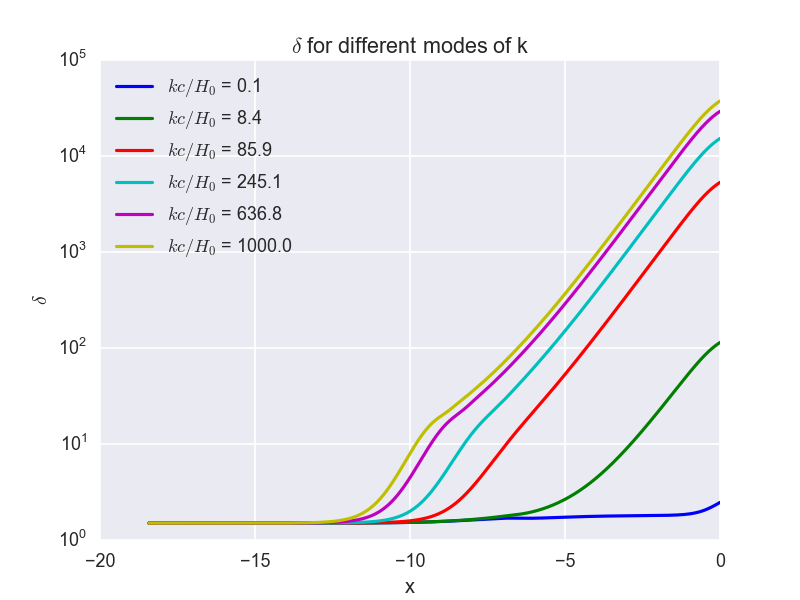
\includegraphics[width=0.5\textwidth]{delta.png}} & 
\subfloat[The figure shows that the survival for male patients are smaller than that for the female patients. The difference is not large, and may not be significant.\label{fig:delta_b}]{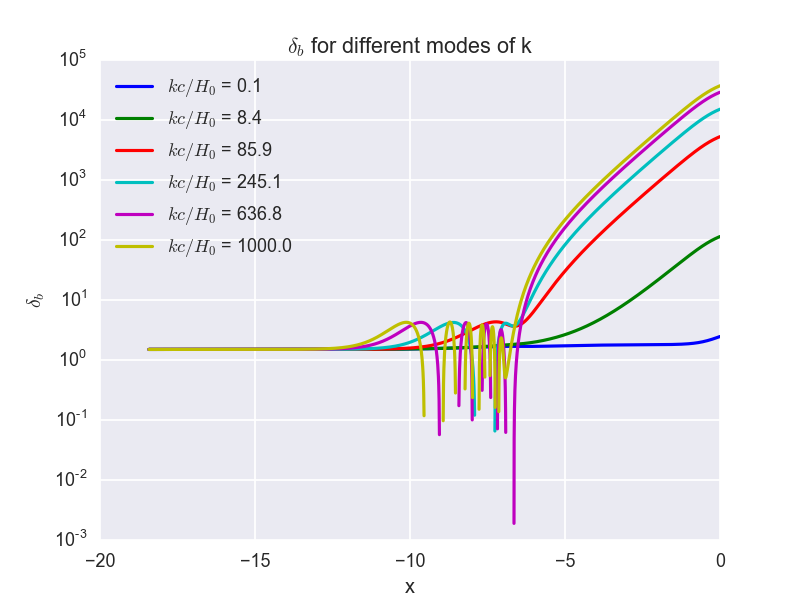
\includegraphics[width=0.5\textwidth]{delta_b.png}} \\
\subfloat[The figure shows that there is a large difference in the survival based on the severity of the ascites of the patient at the start of the observation. The more fluid the patient has, the lower the survival.\label{fig:v}]{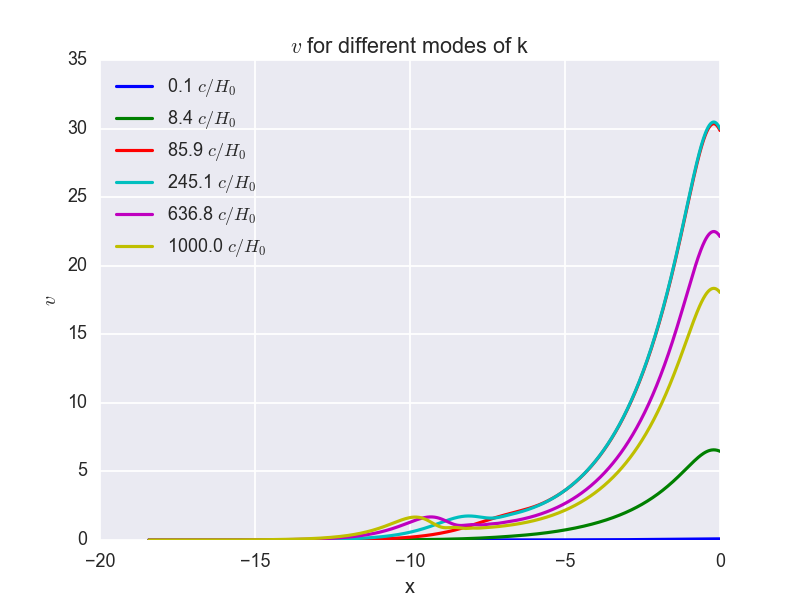
\includegraphics[width=0.5\textwidth]{v.png}} &
\subfloat[The figure shows that the age plays a important role in the survival, with older patients surviving shorter than the younger ones.\label{fig:v_b}]{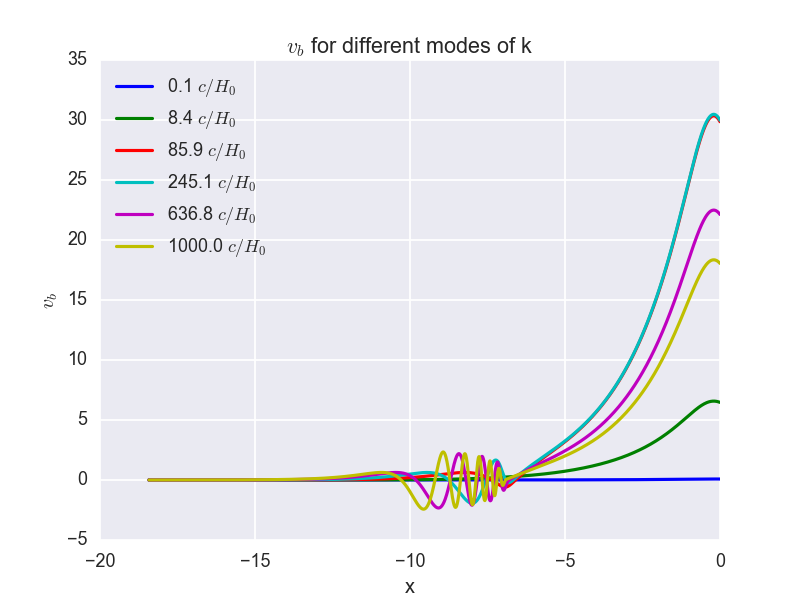
\includegraphics[width=0.5\textwidth]{v_b.png}} 
\end{tabular}
\caption[]{Four figure showing the estimated survival function for different groups.}
\label{fig:delta_v}
\end{figure*}


\begin{figure*}[!htbp]
\centering
\begin{tabular}{@{}ccc@{}}
\subfloat[Survival function for the different treatments. We see that there is some difference, with patients treated with the placebo having lower survival during most of the study. But the difference is very small.\label{fig:Psi}]{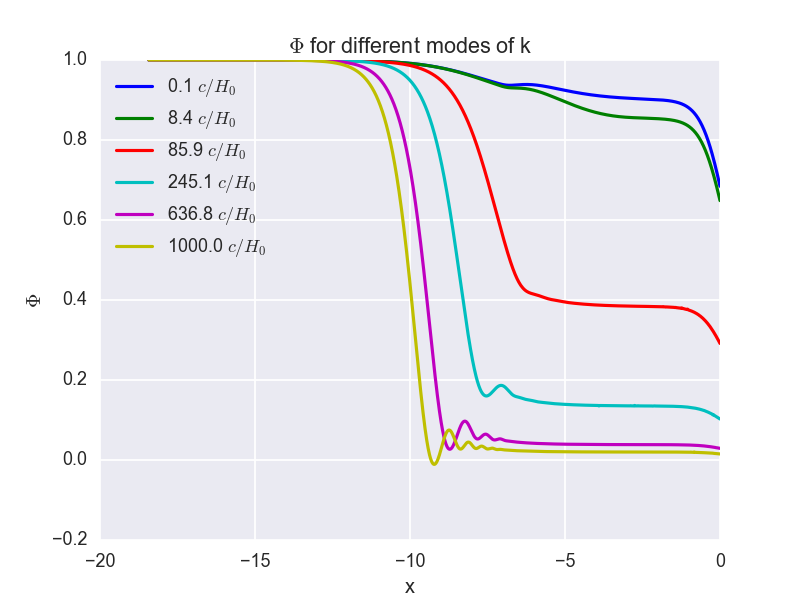
\includegraphics[width=0.5\textwidth]{Phi.png}} & 
\subfloat[The figure shows that the survival for male patients are smaller than that for the female patients. The difference is not large, and may not be significant.\label{fig:Psi}]{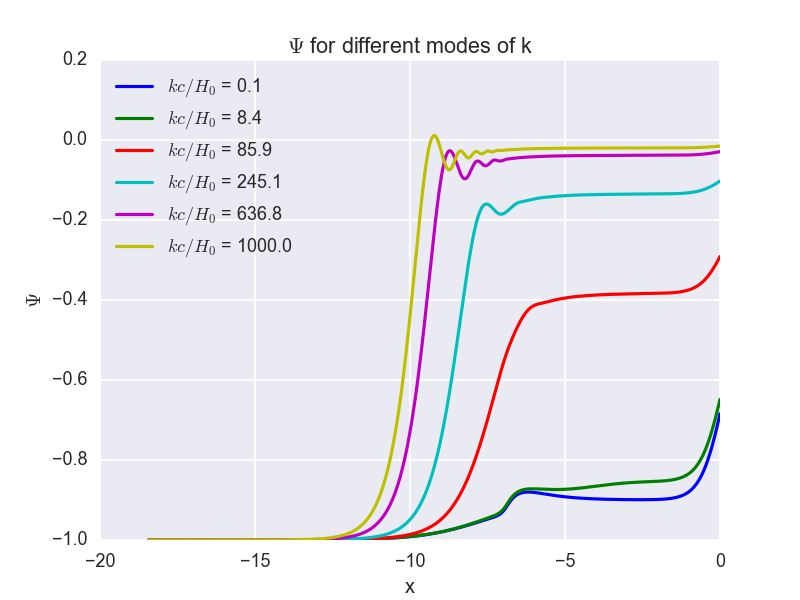
\includegraphics[width=0.5\textwidth]{Psi.png}} 
\end{tabular}
\caption[]{Four figure showing the estimated survival function for different groups.}
\label{fig:psi_phi}
\end{figure*}


\begin{figure}
\centering
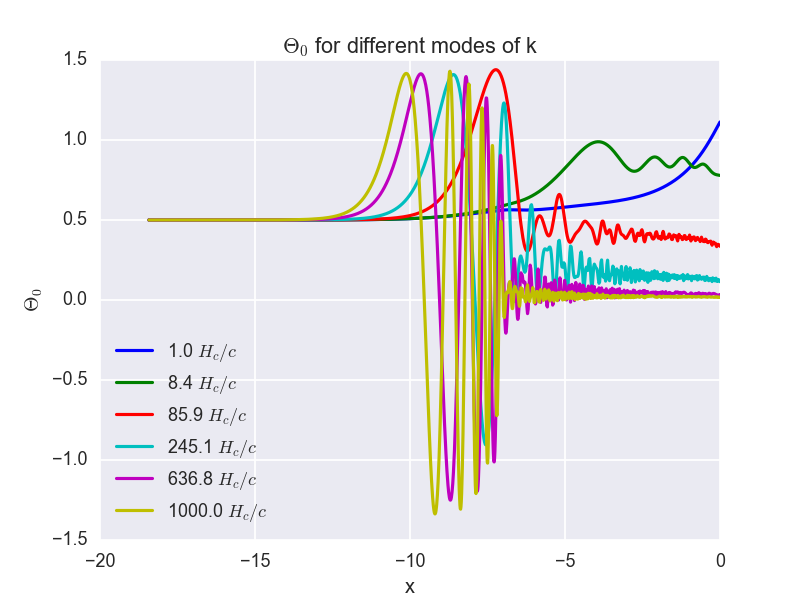
\includegraphics[scale=0.5]{Theta_0.png}
\caption{•}\label{fig:theta}
\end{figure}

\todo[inline]{Notes: As Psi crosses $a_eq$ the transfer function decreases the Psi that have not crossed the horizon to 9/10. If Psi crosses the horizon in the matter dominated regime, it stays constant. This is no longer the case when dark energy takes over, thus the dip in the end (described by the growth function). Growth function is independent of $k$, and is very small in dark energy dom., and we therefore see that perturbations flattens out near $x=0$.

In matter era. delta goes as a. In rad. dom. they grows as well but not as prominent. The pressure from the radiation slows the perturbations down, but as matter begins to dominate, the pressure weakens and the perturbations grow faster.

In rad. dom. the potential is determined by photons, and not dark matter. DM is instead determined by the potential. Potential decays in rad dom.

Seems that modes grows independent of $k$ after crossing the horizon.

The oscillations found in $\Theta_0$ is that makes $\delta_b$ oscillate, due to tight coupling.}

\end{document}

